\usetikzlibrary{calc, arrows.meta}


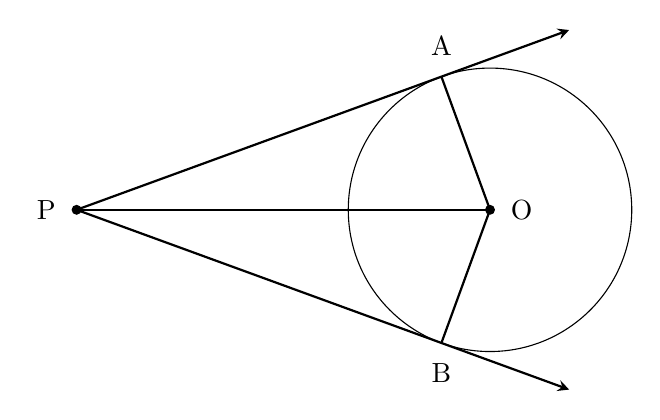
\begin{tikzpicture}[scale=1.5, >=stealth]
    % --- Definitions ---
    % Center O at (0,0)
    \coordinate (O) at (0,0);
    % Radius of the circle
    \def\rad{1.2}
    % External point P (placed to the left)
    \coordinate (P) at (-3.5, 0);

    % --- Calculations ---
    % Calculate the angle for the tangent points A and B
    % Using the property that radius is perpendicular to tangent:
    % cos(theta) = -r / d  (where d is distance PO)
    % The angle is measured from the positive x-axis
    \pgfmathsetmacro{\tangentAngle}{acos(-\rad/3.5)}
    
    % Define Tangent Points A (top) and B (bottom)
    \coordinate (A) at (\tangentAngle:\rad);
    \coordinate (B) at (-\tangentAngle:\rad);

    % --- Drawing ---
    
    % 1. Draw the Circle
    \draw (O) circle (\rad);

    % 2. Draw the Radii (O to A and O to B)
    \draw[thick] (O) -- (A);
    \draw[thick] (O) -- (B);

    % 3. Draw the center line connecting P to O
    \draw[thick] (P) -- (O);

    % 4. Draw Tangent Lines with arrows
    % We extend the line from P through A/B slightly to match the image style
    \draw[thick, ->] (P) -- ($(P)!1.35!(A)$);
    \draw[thick, ->] (P) -- ($(P)!1.35!(B)$);

    % --- Dots ---
    \fill (O) circle (1.2pt);
    \fill (P) circle (1.2pt);

    % --- Labels ---
    % Position labels exactly as shown in the reference image
    \node[right=4pt] at (O) {O};
    \node[left=4pt] at (P) {P};
    \node[above=4pt] at (A) {A};
    \node[below=4pt] at (B) {B};

\end{tikzpicture}